\section{Framework}
\label{sec:framework}

Response surface methodology~\cite{box51response,carley04response}, also known as metamodel-based methods~\cite{barton06metamodel} for stochastic simulations is generally used for optimization~\cite{neddermeijer00response} and calibration~\cite{fadikar17emulation, lamperti18calibration}.
The general idea is to approximate the stochastic objective function (the ``response'') by a low order polynomial function
of the independent variables over a part of the domain.
RSM typically runs in phases. The process starts with a screening experiment, which identifies a subset of
candidate variables, which are most significant in the region of interest.
Next, a first-order model is used to approximate the response, and a line search is used to 
find an improving direction for the objective.
In the second phase, a second-order model is used to approximate the objective, since
usually a response surface has curvature near the optimum.


We denote the agent-based simulation model as a stochastic function, $F(\xi_1, \xi_2, ..., \xi_k)$, of its parameters, assuming a fixed initial condition. In response surface methodology, we generally fit the expected value of this function,
\begin{equation}
f(\xi_1, \xi_2, ..., \xi_k) = \mathbf{E}(F(\xi_1, \xi_2, ..., \xi_k)),
\end{equation}
where $F$ is the stochastic output, given parameters $\xi_1, \xi_2, ..., \xi_k$, and $\mathbf{E}$ denotes expectation. This is appropriate when the goal is optimization or calibration.

However, when we are using the ABM to model a specific observed phenomenon, as is the case in the scenarios described in Section~\ref{section:rooftop}, the real-world data represent only one stochastic realization of the model.
Therefore, instead of taking the expectation, we characterize the behavior of the ABM in terms of the probability of seeing a particular output given a particular
parameter setting. For ease of exposition, we assume that the simulation outputs one continuous variable, $y$, though the
formalism generalizes straightforwardly to multiple outputs. We relate $y$ to the parameters as follows.
\begin{equation}
P(y_{low} < y < y_{high}) = \int P(y_{low} < F < y_{high}|\Xi)P(\Xi),
\label{eqn:output_probability}
\end{equation}
where $\Xi = [\xi_1, \xi_2, ..., \xi_k]$, and $P(\Xi)$ is a prior probability over the parameter space. Thus, the ABM can be
characterized as a discretized probability distribution, using a set of bins denoted by their bin boundaries, $\{[y_0,y_1], [y_1,y_2], ..., [y_{n-1}, y_n]\}$.
The choice of bins depends on the domain of the model. For example, models of contagion processes exhibit sharp
transitions, which are a natural choice for bin boundaries in that case, as we will see in the experiments section. We
refer to this distribution as the \emph{characteristic distribution} for the ABM.

We define the \emph{characteristic distance} between two ABMs as the distance between their characteristic distributions.
\begin{equation}
d(F_1, F_2) := D(P_1(y), P_2(y)). \label{eq:charDist}
\end{equation}
There are multiple valid choices for $D$, such as the (symmetric) KL-divergence, mean-squared distance, total variation distance, earth-mover's distance, etc. Note that this distance is well-defined even if the two ABMs have entirely different parameter spaces, since it is defined only over the output space. Thus it is a fairly general method of comparison. 
For a given observed value, $y_{obs}$, we can also directly compare the 
probabilities assigned by the two models to the corresponding bin.
\begin{equation}
    d_{obs}(F_1, F_2) := P_1(B_{obs}) - P_2(B_{obs}),
\end{equation}
where $B_{obs}$ is the bin within which $y_{obs}$ lies. This directly tells us how much more likely it is to see $y_{obs}$ in one model versus the other.

For a general comparison of the two ABMs in the case where the two ABMs have an overlap in their parameter space (i.e., they have some parameters in common), we can have a more detailed comparison. Let $\Xi_{c}$ be the parameters that the two ABMs have in common. We can partition this subspace of the parameter space into regions based on the most likely bin for $y$ for each parameter setting.
\begin{equation}
    B(\Xi_{c}) = \argmax_B \int_{\Xi \setminus \Xi_{c}} P(B|\Xi)P(\Xi \setminus \Xi_{c}),
\label{eqn:B}
\end{equation}
where $B$ denotes a bin, corresponding to the bin boundaries defined earlier, and $\Xi \setminus \Xi_{c}$ denotes the parameters other than the common parameters. The equation above assigns to each point in the common parameter subspace, a bin corresponding to the most likely output at that point.

Now we define the \emph{disagreement}, $\Delta$, between the two ABMs as the probability of choosing a parameter setting, according to the prior distribution, that results in a difference in the outputs of the two models.
\begin{equation}
    \Delta(F_1, F_2) = \int_{\Xi_{c}} \mathbf{1}(B_1(\Xi_{c}), B_2(\Xi_{c}))P_1(\Xi_{c}),  \label{eq:disagreement}
\end{equation}
where $\mathbf{1}(B_1(\Xi_{c}), B_2(\Xi_{c}))$ is an indicator function that is 1 if $B_1(\Xi_{c}) = B_2(\Xi_{c})$ and 0 otherwise. $\Delta$ gives the total probability, over the subspace $\Xi_c$, that the outputs of the two ABMs will fall into different bins. Note that $\Delta$ is a directed measure, since $\Delta(F_1, F_2) \ne \Delta(F_2, F_1)$.

There are various ways to compute the integral in equation~\ref{eqn:B}. The typical approach in simulation
science is to use adaptive experiment designs~\cite{perez02adaptive}. Here we propose a machine learning approach based on active learning. The general idea is to train a multi-class classifier, where a class corresponds to a bin, for each model. Since the simulations can often be expensive to run, an active learning approach can help minimize the number of times the simulation has to be run.
The classifiers are used to estimate $B(\Xi_{c})$ for each ABM.
Once the classifiers have been trained, we can use them to estimate $\Delta$.

\begin{figure}
    \centering
    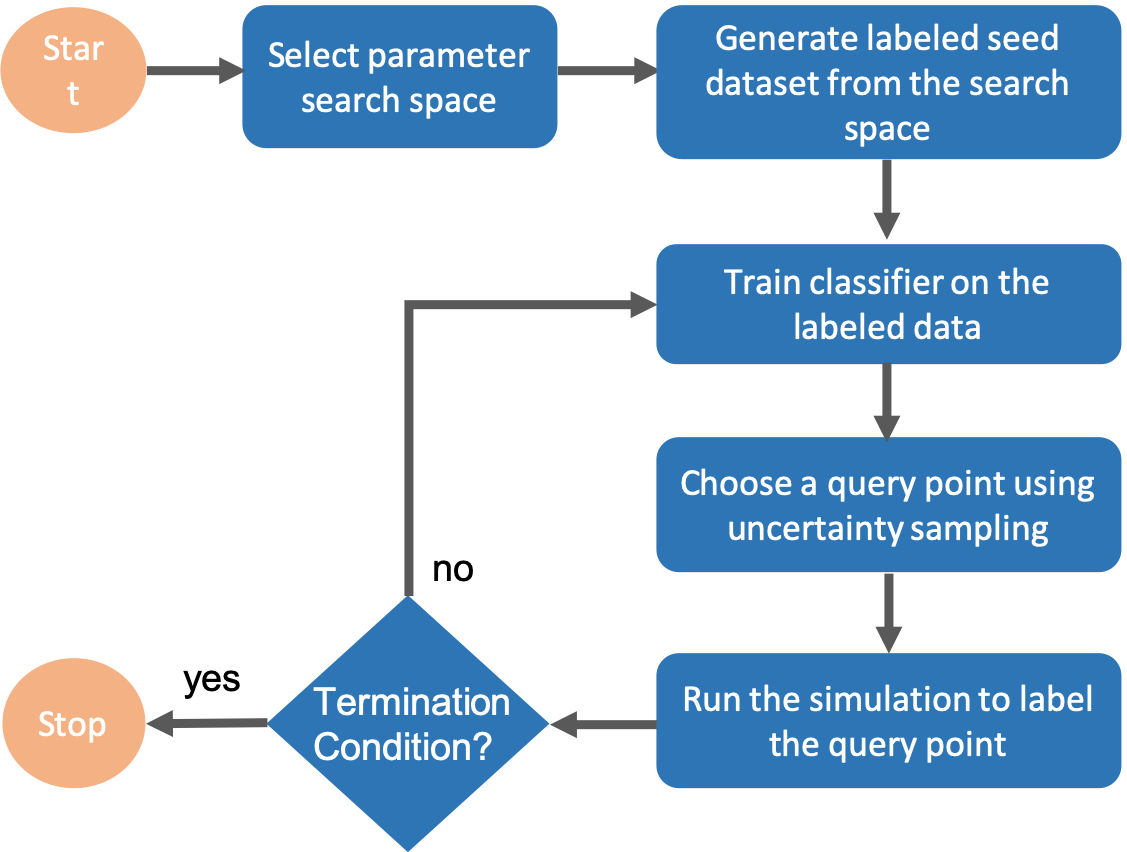
\includegraphics[width=0.4\textwidth]{AAMAS20Template-submission/figures/workflow1.png}
    \caption{Overview of the presented methodology - A common set of parameters is chosen from both ABMs and an active learning framework is implemented to learn the decision boundary that separates the bins. }
    \label{fig:workflow}
\end{figure}

The active learning approach to training the classifier involves running the simulation in a loop with the classifier. In each round, the simulation is run to generate additional labeled points for the classifier. Then the classifier is trained on the updated data set and we do uncertainty sampling~\cite{lewis94sequential} in the parameter space to generate new parameter settings where the simulation is to be evaluated in the next round. The process stops when the labels generated by the simulation agree with the labels generated by the classifier, as illustrated in Figure~\ref{fig:workflow}.
In the particular scenario we study below, we will see that we can exploit domain semantics to generate multiple useful labeled points from one query. We continue below by first describing the models that we built for studying rooftop solar panel adoption in rural Virginia, USA, and the model we compare with, which was built to study solar panel adoption in San Diego, California, USA. Then we will describe how this framework is instantiated for these models.